\chapter{Knowledge Tracing Based Exercise Recommendation Model }

% **************************** Define Graphics Path **************************
\ifpdf
  \graphicspath{{Chapter4/Figs/Raster/}{Chapter4/Figs/PDF/}{Chapter4/Figs/}}
\else
  \graphicspath{{Chapter4/Figs/Raster/}{Chapter4/Figs/PDF/}{Chapter4/Figs/}}
\fi

\section{Research Motivation}
%随着当今技术的飞速发展,数据量也与日俱增,人们越来越感觉在海量数据面前束手无策。正是为了解决信息过载的问题,人们提出了推荐引擎技术。推荐系统通过用户的历史行为或者用户的兴趣偏好或者用户的人口统计学特征来送给推荐算法,然后推荐系统运用推荐算法来产生用户可能感兴趣的项目列表,同时用户对于搜索引擎是被动的。目前个性化推荐技术被广泛应用于各个行业,它大大节省了用户获取信息的成本,也方便了信息提供商对用户的定向信息推送,因此大大加速了社会的信息交流效率,从而推动了传媒、娱乐、教育等基于信息交流的行业的发展。在教育领域,推荐系统的应用仍停留在较为初级的阶段,很多情况下还依赖人工筛选教育资源进行推荐,这种推荐方式效率低、成效差,且出于成本的原因也无法覆盖到所有的学生。随着推荐系统技术的成功应用和教育行业的进一步成熟,将以往通过人工实现的教育资源推荐系统改用智能化技术来进行的阻力越来越小。在国家提倡智慧教育、精准教学、智慧学习的背景下,一款成熟的具备实用价值的自适应习题推荐系统成为教育业者的期待。

%本章的目的是基于前两个章节所挖掘出的习题知识点和知识状态进行习题推荐,其核心是基于学生的知识状态,寻找出对学生当前知识掌握度改善最大的习题进行推荐。习题推荐以查漏补缺为目的,因此获取学生的知识状态和习题涉及的知识点是本章前提。但是目前的习题库往往过于庞大,因此,从海量的习题推荐资源中直接应用推荐算法会出现效率较低的情况,不利于商业化大规模部署。在匹配阶段,根据用户特征,从海量的习题库中,快速筛选出一部分潜在适合的习题作为粗筛集合。在排序阶段,将提出的推荐模型应用于粗筛习题集,输出一个按照优先级排序的推荐习题集列表。

With the rapid development of today's technology, the amount of data is increasing day by day, and folks increasingly feel helpless in the face of massive amounts of data. It is precisely to solve the problem of information overload that people propose the recommendation engine technology. The recommendation system sends the recommendation algorithm to the recommendation algorithm through the user's historical behavior or the user's interest preferences, or the user's demographic characteristics, and then the recommendation system uses the recommendation algorithm to generate a list of items that the user may be interested in. At the same time, the user is passive to the search engine. At present, personalized recommendation technology is widely used in various industries. It greatly saves the cost for users to obtain information, and it also facilitates information providers to push targeted information to users. Therefore, it dramatically accelerates social information exchange efficiency, thereby promoting media and developing industries based on information exchange, such as entertainment and education. In the education field, the application of the recommendation system is still at a relatively primitive stage.

In many cases, it still relies on manual screening of educational resources for a recommendation. This recommendation method is inefficient, poorly effective, and cannot cover all of them due to cost reasons. With the successful application of the recommendation system technology and the further maturity of the education industry, the resistance to intelligent technology in the education resource recommendation system implemented manually in the past is decreasing. In the context of the country's promotion of smart education, precise teaching, and smart learning, a mature and practical self-adaptive exercise recommendation system has become the education industry's expectation. This chapter proposes an exercise recommendation model based on students' knowledge mastery to improve education and teaching.

This chapter aims to recommend exercises based on the knowledge points and knowledge states of the exercises mined in the previous two chapters. The core of this chapter is to find the exercises that improve the students' current knowledge the most based on their knowledge states. The exercises are recommended to check the gaps, so it is a prerequisite for this chapter to obtain the students' knowledge status and the knowledge points involved in the exercises.  However, the current exercise database is often too large, so the direct application of recommendation algorithms from the massive exercise recommendation resources will result in low efficiency, which is not conducive to large-scale commercial deployment. A portion of potentially suitable exercises is quickly filtered out from the massive exercise database as a coarse screening set based on user characteristics in the matching phase. In the sorting phase, the proposed recommendation model is applied to the coarse sieved exercise set, and a list of recommended exercises set is output in the order of priority.

\section{Proposed Model}
%推荐系统本质上就是一个信息过滤系统,目前常见的工业推荐系统往往具备若干过滤、排序等多个环节,每个环节逐层过滤,最终从海量的物料库中筛选出几十个用户可能感兴趣的物品推荐给用户。推荐系统作为一种解决用户信息过载的方式,通过分析用户的行为数据、历史记录等等来建立用户画像,再根据用户个性化模型推荐他们感兴趣的推荐项。在传统的推荐系统中,采用的模型一般是基于矩阵分解模型的模型,例如SVD+、BPR、 因子分解机(FM)等等,随着深度学习研究的兴起,基于深度学习模型的深度推荐模型技术也逐渐发展起来。目前已经有一些模型用深度学习来表征推荐项目的高阶特征,例如Deep&Wide、DeepCross、DeepFM等。深度推荐模型由于其对隐藏特征的建模能力,在推荐精度上有部分提升。但是深度推荐算法往往会产生较大的计算开销,直接应用全阶段深度推荐模型不切实际,因此可以采用基于匹配-排序双阶段的推荐模型,利用开销较低的匹配算法来进行推荐项近似筛选,产生候选推荐项目集合。匹配阶段的核心任务是从海量习题库中快速获取一批候选习题库,要求是快和尽可能的准。这一层通常有丰富的策略和算法,用来确保多样性,为了更好的推荐效果,需要对算法进行速度与精度的权衡。在排序阶段再应用推荐算法进行推荐项的打分或者优先级排序,进行精细化排序。它会利用习题、用户以及习题-用户交叉特征,然后通过复杂的机器学习或者深度学习模型进行打分排序,这一层的特点是计算复杂但是结果更精准。

A recommendation system is essentially an information filtering system. Currently, common industrial recommendation systems often have several filters, ranking, and other multiple links, each filtering layer by layer and eventually filtering out dozens of items that may be of interest to users from a massive library of materials to recommend to users. As a method to solve user information overload, the recommendation system builds user portraits by analyzing user behavior data, historical records, etc., and then recommends recommendation items that they are interested in based on the user's personalized model. In traditional recommendation systems, the models used are generally models based on matrix factorization models, such as BPR~\cite{rendle2012bpr}, factorization machines (FM)~\cite{koren2008factorization} and weighted matrix factorization(WMF)~\cite{hu2008collaborative}, etc. As deep learning research gradually becomes popular, deep recommendation model technology is gradually developed based on deep learning models. There are already some models that use deep learning to characterize the high-level features of recommended items, such as Deep\&Wide~\cite{cheng2016wide}, DeepCross~\cite{shan2016deep}, DeepFM~\cite{guo2017deepfm}, etc. The deep recommendation model has a partial improvement in recommendation accuracy due to its ability to model hidden features. However, in-depth recommendation algorithms often incur large computational overhead, and it is impractical to apply the full-stage in-depth recommendation model directly. Therefore, a recommendation model based on a matching-ranking two-stage can be used, and a matching algorithm with lower overhead can be used to approximate recommendation items. , Generate a set of candidate recommendation items. The matching phase's core task is to quickly obtain a pool of candidate exercises from a massive library of exercises, and the requirement is to be fast and as accurate as possible. This layer usually has a rich set of strategies and algorithms used to ensure diversity, and the algorithms need to be traded off between speed and accuracy for better recommendation results. The recommendation algorithm is then applied in the ranking stage to score or prioritize the recommended items for refined ranking. It will use the exercise, user, and exercise-user crossover features and then perform scoring and ranking by complex machine learning or deep learning models, characterized by a complex calculation but more accurate results at this layer.

\subsection{Algorithm Overview}
%本章提出一个基于Matching-Ranking双阶段的数学习题推荐模型。考虑到待推荐的习题库较为庞大,直接应用知识追踪推荐模型会产生较大的计算开销。本节提出一种基于多策略习题筛选的方式,先对习题应用计算开销较低的习题筛选策略生成习题推荐候选集,然后再对候选推荐习题应用推荐算法。

This chapter proposes a recommendation model based on Matching-Ranking two-stage for Math exercises. Considering that the recommended database of exercises is relatively large, the knowledge tracing recommendation model's direct application will generate a high computational cost. This section proposes a method based on multi-strategy exercises screening. The exercise screening strategy with the low computational cost is first applied to the exercises to generate the exercise recommendation candidate set, and then the recommendation algorithm is applied to the candidate recommended exercises.

%整个模型的介绍如下:
%1. 召回。这部分的作用是生成一系列候选推荐习题。本文应用了多路召回策略,即应用多种召回策略分别形成对应的子候选集合再应用融合方法将它们合并为一个候选集合。文中分别应用了基于协同过滤、基于统计信息和基于用户偏好的三种匹配策略,应用加权平均的方法进行排序融合。

%2. 排序。这部分的作用是应用知识追踪推荐模型到之前匹配阶段生成的候选推荐习题集,根据习题回答预测的情况进行习题推荐度排序,生成一个最终的习题推荐列表。

The overview of the entire model is as follows:
\begin{enumerate}
  \item Matching: The purpose of this part is to generate a series of candidate recommendation exercises. In this thesis, a multi-path matching strategy is applied, in which multiple matching strategies are applied to form corresponding sub-candidate sets and then merged into a candidate set by the merging method. Three matching strategies based on collaborative filtering, statistical information, and user preferences are respectively applied in this thesis, and the weighted average method is used for ranking and merging.
  \item Ranking: The purpose of this part is to apply the knowledge tracing recommendation model to the candidate recommended exercise set generated in the previous matching stage, sort the exercise recommendation degree according to the prediction of the exercise answer, and generate a final exercise recommendation list.
\end{enumerate}

The structure of the recommendation system is like \figurename{\ref{fig:ch4-model-architecture}}

\begin{figure}[htbp!]
  \centering
  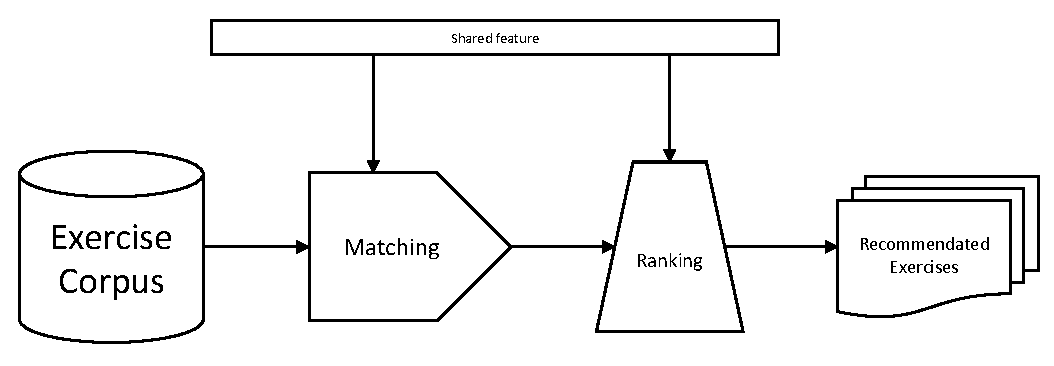
\includegraphics[width=0.9\textwidth]{ch4-model-architecture.pdf}
  \caption{The architecture of recommendation system}\label{fig:ch4-model-architecture}
\end{figure}

\subsection{Matching Phase}
%本推荐模型的第一阶段为匹配,匹配层的目的是在确保一定准确度的情况下快速筛选出候选的推荐习题集合。匹配有多种策略来应对不同的应用场景。例如,与新闻推荐算法等相比,习题和用户的知识状态都是较为规则化的向量数据,计算习题、用户以及习题-用户交叉特征相似度相对简单,因此可以利用相似度匹配来应用协同过滤策略进行推荐项匹配。用户的历史回答错误错习题、统计的容易答错的习题等对于学生检查知识掌握完整度以及更正误区具有较大意义,因此筛选错误率较高的习题也可以作为一种匹配策略。在匹配阶段,可以应用不同的自适应参数或算法来控制候选习题集的大小,以适配原始数据集和推荐系统部署环境。

%采用不同的匹配策略,所对应的推荐侧重点也不同。一方面,不同的匹配策略会带来不同的推荐结果并忽略一部分推荐结果,例如,如果重视热门习题,则将做的人最多的习题作为匹配的结果,如果重视容易出错的习题,则将错误率较高的习题作为匹配的结果,如果重视基于相同兴趣的推荐,则将协同过滤作为匹配的结果。单独采用某一种匹配策略往往具有一定的缺陷,例如采用热门度作为匹配策略,会使得冷门习题几乎得不到被匹配的机会,导致推荐概率失衡,而采用错误率作为匹配策略则会无法匹配所有学生的知识情况。因此单独的匹配策略会丢失大量的推荐信息。另一方面,设计匹配层的时候,``计算速度''与``匹配率''这两个指标是相互矛盾的,也就是说在提高计算速度的时候需要尽量简化匹配策略,这就会导致匹配率不尽人意,同样的,需要提高匹配率时就需要复杂的匹配策略,这样计算速度肯定会相应的降低。在权衡两者后,目前工业界普遍采用多个简单的匹配策略叠加的``多路匹配策略''。``多路匹配策略''就是指采用不同的策略、特征或者简单模型,分别匹配一部分候选集,然后再把这些候选集进行合并、过滤等操作然后供后续排序模型使用的策略。多路匹配综合了多种匹配策略,结合了各个匹配策略的优点。在多路匹配中,每个策略之间毫不相关,所以一般可以写并发多线程同时进行。在实际的生产环境中,可以采取节点集群多线程地来进行召回操作,具备大规模商业应用的前景。

%本节提出一个多路习题推荐项匹配模型,该模型采用了基于热门度、用户兴趣、专家推荐习题、易错题、用户错题集和协同过滤等多个召回策略作为子召回策略,每个子召回策略都基于可学习的参数用于控制该召回策略的权重。当所有的召回策略都返回子召回习题集合后,通过基于加权融合的算法来进行习题的融合、过滤等步骤。其结构如图所示。

The first stage of this recommendation model is matching. The purpose of the matching layer is to quickly filter out a set of the candidate recommended exercises while ensuring a certain degree of accuracy. There are multiple strategies for matching to deal with different application scenarios. For example, compared with news recommendation algorithms, the exercises and the user's knowledge state are more regularized vector data. It is relatively simple to calculate the similarity of exercises, users, and exercise-user cross-features. Accordingly, similarity matching can be used to apply collaborative filtering. The strategy matches recommended items. The user's historical answers to wrong exercises and statistically easy to answer exercises are of great significance for students to check their knowledge's completeness and correct their misunderstandings. Therefore, screening exercises with a higher mistaken rate can also be used as a matching strategy. Different adaptive parameters or algorithms can be applied to control the candidate problem's size to adapt to the original dataset and the recommended system deployment environment in the matching stage.

With different matching strategies, the corresponding recommendation focuses are also different. On the one hand, different matching strategies will lead to different recommendation results and ignore part of the recommendation results. For example, if the most popular exercises are emphasized, the exercises with the most individuals' records will be regarded as the matching results. If the exercises that are prone to errors are emphasized, errors will be regarded as the matching result. The exercises with a higher rate are used as the matching result. If the recommendation based on the same interest is emphasized, collaborative filtering will be used as the matching result. Adopting a certain matching strategy alone often has certain drawbacks. For example, using popularity as a matching strategy will make unpopular exercises almost impossible to be matched, resulting in an imbalance in the recommendation probability, while using the mistaken rate as a matching strategy will fail to match all students' knowledge mastery proficiency. Therefore, a single matching strategy will lose a lot of recommendation information. On the other hand, when designing the matching layer, the two indicators of ``calculation speed'' and ``matching rate'' are contradictory. The matching strategy needs to be simplified as much as possible when the calculation speed is increased. As a result, the matching rate is unsatisfactory. Similarly, when the matching rate needs to be improved, a complex matching strategy is required. Accordingly, the calculation speed will definitely be reduced. After weighing the two, the current industry generally adopts a "multiplex matching strategy" in which multiple simple matching strategies are superimposed. The "multiplex matching strategy" refers to a strategy that uses different strategies, features, or simple models to match a part of the candidate set, and then merges, filters, and other operations on these candidate sets, and then uses them for subsequent sorting models. Multiplex matching integrates multiple matching strategies and combines the advantages of each matching strategy. In multiplex matching, each strategy is irrelevant. Accordingly, it is generally possible to write multiple concurrent threads at the same time. In the actual production environment, the node cluster can be used for multi-threaded matching operations, which has the prospect of large-scale commercial applications.

This section proposes a multiplex exercise recommendation item matching model. The model uses multiple matching strategies based on popularity, user interest, expert recommendation exercises, error-prone questions, user error question sets, and collaborative filtering as sub-matching strategies. Matching strategies are based on learnable parameters to control the weight of the matching strategy. After all matching strategies have returned to the sub-matching exercise set, the exercises are merged and filtered through the weighted merging algorithm. Its structure is shown in~\figurename{\ref{fig:ch4-matching}}.

\begin{figure}[htbp!]
  \centering
  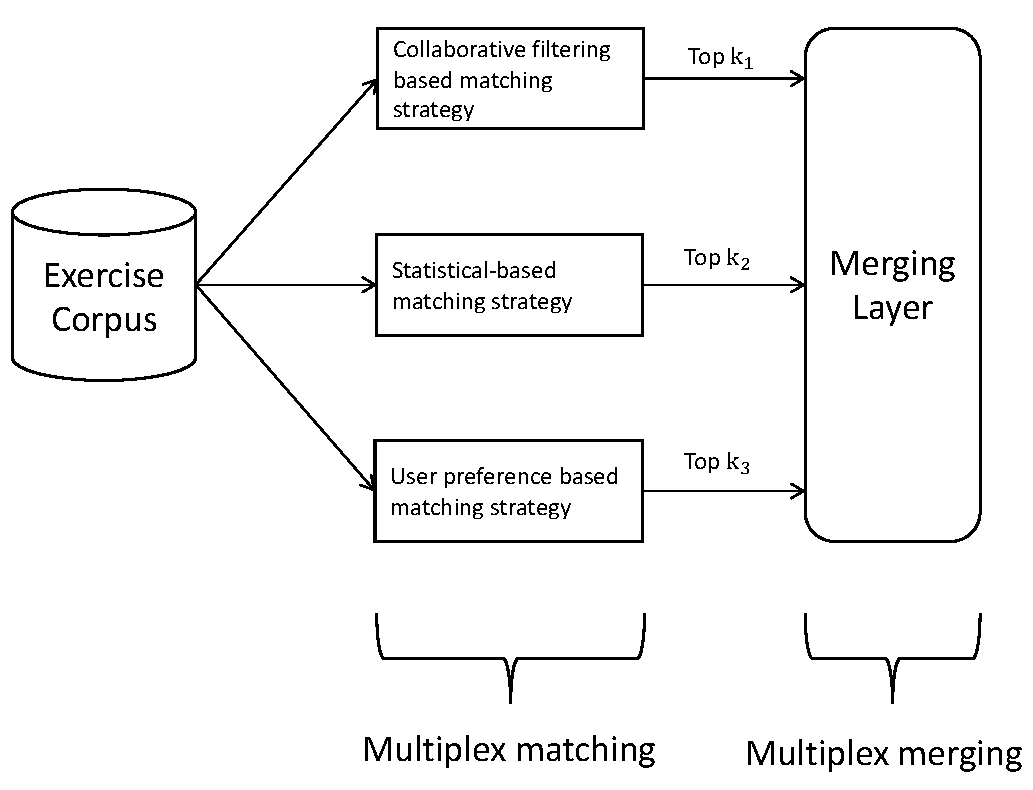
\includegraphics[width=0.8\textwidth]{ch4-model-matching.pdf}
  \caption{The multiplex matching method}\label{fig:ch4-matching}
\end{figure}

\subsubsection{Student-Exercise Collaborative Filtering Based Matching Strategy}
%协同过滤是multiplex matching中的其中一个匹配策略,对于数学习题来说,由于习题已经经过知识点标注,因此可以根据知识点重合程度来计算相似度。同时,对于学生,在知识追踪阶段获取了学生的知识状态表征向量,因此也可以根据该向量计算学生的知识掌握相似度。本节提出一个基于Student-Exercise两阶段的协同过滤算法,该算法先计算学生的相似度,获取相关的习题,再根据这些习题计算相似的习题加入候选集,经过该方法计算的习题集相对而言较为完备,防止出现经过由于相似用户较少而出现的推荐项目稀疏的问题。

%传统基于用户的协同过滤根据模型选择的用户特征计算用户间的相似度,依据相似度来判定用户的状态相似度,并将相似度最高的前几名用户作为该用户的最近邻居用户。邻居用户集合的构建是协同过滤算法重要前提和基础。对于相似用户的计算方法,目前大多数个性化推荐系统主要采用的有:余弦相似性、修正的余弦相似性、皮尔森相关系数~\cite{Novotn__2018},其中余弦相似性是计算两名用户评分向量在向量空间模型中的向量夹角的余弦值,用评分向量夹角的余弦值大小表示用户间的相似性。而修正的余弦相似性主要是解决用户受自身或者其它因素影响导致评分数据不稳定的问题,相较于余弦相似性计算用户间的相似度,修正的余弦相似性计算由于考虑因素较多所以更为准确一些。因为余弦相似度计算方法过于粗糙,未考虑到用户受自身或者其它因素影响因素对用户间相似性的影响,所以更多的基于用户的协同过滤推荐系统选择采用修正的余弦相似性方法计算用户间的相似度。其公式如下所示。其中\(\mathbf{S}^u=(S^u_1,S^u_2,\ldots,S^u_n)\)、\(\mathbf{S}^v=(S^v_1,S^v_2,\ldots,S^v_n)\)分别代表由知识追踪模型输出的用户\(u\)、\(v\)的的知识状态表征向量。

%计算出学生的相似度之后,可以设定一个相似度阈值\(\tau_{simu}\)作为相似学生的筛选标准。对于用户\(u\),所有的相似用户\(\mathbf{U}_{sim}={i|sim(u,i)>\tau_{simu}}\)。为了获取相似的习题,选择\(\mathbf{U}_{sim}\)中的用户的错题集或者收集题集。将用户\(i\)的错题集合和收藏习题集合分别表示为\(\mathbf{E}_{i}^err\)和\(\mathbf{E}_{i}^fav\)。最终将符合要求的相似用户的错题集合和收藏习题集合进行归并和去重,即得到目标习题集合。

Collaborative filtering is one of the matching strategies in multiplex matching. For math learning questions, because the exercises have been labeled with knowledge points, the similarity can be calculated according to the degree of overlap of the knowledge points. Simultaneously, for students, the student's knowledge state representation vector is obtained in the knowledge tracing stage, so the students' knowledge mastery similarity can also be calculated based on this vector. This section proposes a two-stage collaborative filtering algorithm based on Student-Exercise. The algorithm first calculates students' similarity, obtains related exercises, and then calculates similar exercises based on these exercises and adds them to the candidate set. The exercise set calculated by this method is relatively The language is relatively complete to prevent sparse recommendation items that appear due to fewer similar users.

Traditional user-based collaborative filtering calculates the similarity between users, determining the similarity of the user's state according to the similarity, and uses the top users with the highest similarity as the user's nearest neighbors. The construction of the neighbor user set is an important premise and foundation of the collaborative filtering algorithm. For similar users' calculation methods, most of the current personalized recommendation systems mainly use cosine similarity, modified cosine similarity, and correlation similarity. Cosine similarity is to calculate the cosine value of the angle between the two users' rating vectors in the vector space model, and the cosine value of the angle between the rating vectors is used to express the similarity between users. The modified cosine similarity is mainly to solve the problem that users are affected by their own or other factors, and the scoring data is unstable. Compared with the cosine similarity calculation of the similarity between users, the modified cosine similarity calculation is more important because of more considerations. Be more accurate. Because the cosine similarity calculation method is too rough and does not consider the user's influence or other factors on the similarity between users, more user-based collaborative filtering recommendation systems choose to use the modified cosine similarity method to calculate the user-to-user similarity. The similarity. The formula is~\ref{fml:ch4-user_similarity}, where \(\mathbf{S}^u=(S^u_1,S^u_2,\ldots,S^u_n)\), \(\mathbf{S}^v=(S^v_1,S^v_2,\ldots, S^v_n)\) represent the representation vectors of the knowledge state of users \(u\) and \(v\) output by the knowledge tracing model, respectively.

\begin{align}\label{fml:ch4-user_similarity}
  \begin{split}
    sim(u, v) & =\frac{\mathbf{S}^u \cdot \mathbf{S}^v}{|\mathbf{S}^u|\cdot |\mathbf{S}^v}                                                                 \\
    & =\frac{\sum\limits_{i = 1}^{n}{S^u_i\cdot S^v_i}}{\sqrt{\sum\limits_{i = 1}^{n}{{S^u_i}^2}}\cdot\sqrt{\sum\limits_{i = 1}^{n}{{S^v_i}^2}}}
  \end{split}
\end{align}

After the similarity of students is obtained, a similarity threshold \(\tau^{simuser}\) can be set as the screening criterion for similar students. For user \(u\), the similar user set can be denoted as \(\mathbf{U}_{sim}\), the calculation of which is formula~\ref{fml:ch4-simuserset}. In order to obtain similar exercises, select the user's mistaken exercise set or favorites exercise set in \(\mathbf{U}_{sim}\). Denote Aggregation of the mistaken exercise set and favorites exercise set of the user \(i\) as \(\mathbf{E}_{i}\). Finally, the set of wrong questions and the set of favorite exercises of similar users that meet the requirements are merged and deduplicated to obtain the target exercises set.

\begin{align}
  \mathbf{U}_{sim} & =\{i|sim(u,i)>\tau^{simuser}\}  \label{fml:ch4-simuserset}
\end{align}

The general algorithm is as~\ref{alg:ch4-CF}:
\begin{algorithm}[htbp!]
  \caption{Student-exercise collaborative filtering algorithm}\label{alg:ch4-CF}
  \begin{algorithmic}
    \REQUIRE~~\\
    The target student \(u\); \\
    The similarity threshold \(\tau^{simuser}\)
    The student knowledge state representing matrix for all \(N\) students, \(\mathbf{S}=\{\mathbf{S}^1,\mathbf{S}^2,\ldots,\mathbf{S}^N\} \);\\
    The mistaken/favorite exercise sets of all students \( \mathbf{E}=\{\mathbf{E}_1,\mathbf{E}_2,\ldots,\mathbf{E}_N\} \) \\
    \ENSURE~~\\ %算法的输出:Output
    The output exercise set \(\mathbf{E}^{(UCF)} \)
    \STATE~Calculate the similar user set \(\mathbf{U}_{sim}=\{i|sim(u,i)>\tau^{simuser}\}  \)
    \STATE~Aggregate the mistaken/favorites exercise set of users in \(\mathbf{U}_{sim}\), \(\mathbf{E}^{(UCF)}=\sum\limits_{i \in \mathbf{U}_{sim}}{\mathbf{E}_{i}}\)
    \RETURN~~\(\mathbf{E}^{(UCF)} \); %算法的返回值
  \end{algorithmic}
\end{algorithm}

The exercise \(E_j\) of in students exercise set \(\mathbf{E}_i\) recommendation score denoted as \(S^{(UCF)}\) is defined by formula~\ref{fml:ch4-ucfscore}. The strategy weight is denoted as \(w^{(UCF)}\).
\begin{align}\label{fml:ch4-ucfscore}
  S^{(UCF)}_{i,j} = sim(u,i)
\end{align}


\subsubsection{Popularity-based Matching Strategy}
%本部分基于运动语料库的统计数据提出了推荐项召回策略。 该策略将演习的受欢迎程度,错误回答率和专家推荐作为推荐得分的计算因素。其中热门度是一个结合习题被回答过的次数和习题被用户收藏次数的特征。它将被回答过过次数最多的习题和被收藏次数最多的习题筛选出来进行综合加权排序,记习题排序综合权重为\(w_{(pop)}\),被回答次数以及对应权重分别记作\(S{(\#ans)}\)和\(w_{(\#ans)}\),被收藏次数以及对应权重分别记作\(S_{favorite}\)和\(w_{favorite}\),被回答错误的次数以及对应权重分别记作\(S_{(\#wrong)})和\(w_{(\#wrong)}\),是否经过专家推荐以及对应权重分别记作\(S_{expert}\)和\(w_{expert}\)。则综合权重计算公式如下。

%\(S_ {ans} \)的计数将执行用户重复数据删除,也就是说,每个用户的重复答案数仅计算一次,以防止单个用户重复回答而导致数据失真。 实际上,它等于已回答问题的用户在总用户中所占的比例。 同样,\(S_ {favorite} \)和\(S_ {wrong} \)的计算将遵循此统计方法。 因此,每个值都经过归一化,每个值的范围从0到1。对于专家推荐值\(S_ {expert} \),它表示推荐分数,并且值的范围是0-1。 对于没有专家推荐值的练习,默认值为0。

%计算出\(S_{pop}\)后,将习题按照\(S_{pop}\)的大小从大到小排序,将前\(K_{SMS}\)个项目作为推荐项召回集。此处的\(K_{SMS}\)是一个可调的超参数,可以根据业务的需要进行调整,来控制推荐的侧重点。可以根据业务的需要进行调整,来控制推荐的侧重点。

This section proposes a recommendation item matching strategy based on the statistical popularity of the exercise corpus. The strategy focus on the exercises' popularity consists of click rate, favorite rate, mistaken rate, and expert recommendation. Click rate is a feature that combines the number of times the exercises have been answered. The favorite rate is the number of times users favorite the exercises. Mistaken rate is the number of mistakenly answering to the exercise. The comprehensive popularity score is denoted as \(S^{(PMS)}\), of which the number of answering record to the exercises and the corresponding weight is denoted as \(N^{(SA)}\) and \(w^{(SA)}\), the number of favorites to the exercise and the corresponding weight are respectively denoted as \(N^{(SF)}\) and \(w^{(SF)} \), the times of incorrect answers record and the corresponding weight are denoted as \(N^{(SW)}\) and \(w^{(SW)}\). The weight value is adjusted according to the focus of the source. Furthermore, expert-recommended exercises should be concerned, which are some excellent exercises in the set of exercises manually recommended by industry practitioners with educational experience based on experience, with a recommendation score \(S^{(EX)}\) and respective weight \(w^{(EX)}\). Then the comprehensive popularity calculation formula of one exercise is~\ref{fml:ch4-pop}.
\begin{align}
  S^{(PMS)} & = w^{(SA)}\cdot \sigma(N^{(SA)})+w^{(SF)}\cdot\sigma(N^{(SF)})+w^{(SW)}\cdot\sigma(N^{(SW)})+w^{(EX)}\cdot S^{(EX)}\label{fml:ch4-pop}
\end{align}
Where \(\sigma(\cdot)\) represents the sigmoid function.

After calculating \(S^{(PMS)}\), sort the exercises according to the size of \(S^{(PMS)}\) from large to small, and filter the first \(K^{(PMS)}\) items as the recommended item matching set. Here \(K^{(PMS)}\) is an adjustable hyperparameter, which can be adjusted according to the needs of the business to control the recommended focus and can be adjusted according to the needs of the business to control the recommended focus.

\subsubsection{User-Preference based Matching Strategy}
%本节提出基于用户偏好的推荐项目召回策略,该策略将用户做过的错题、收藏过的习题作为召回项。通过这种方式,可以实现用户对习题推荐结果的定制化。在充分实现智能化推荐的同时,让用户可以基于自己对于知识状态的评估来选择练习题。用户回答错误的习题,设定回答错误次数为\(n_a\),则掌握度计算为\(S_{userwrong}=\frac{1}{n_a}\)。在习题推荐系统中,为了增强用户对于知识的记忆和掌握程度,多次错误的习题的优先级应当更高。而收藏的习题是用户自己选择,是用户主动对自己知识状态的评估,收藏与否只有两个状态0和1,记做\(S_{userfav}\)。此处设定错题权重为\(w_{userwrong}\),收藏的习题权值为\(w_{userfav}\),则习题的综合优先级\(S_{user}\)的计算公式为

%计算出S_{user}值后,将用户错题集和收藏习题集中的习题按照改值进行排序,筛选出前\(K_{UMS}\)个,其中\(K_{UMS}\)为一个可调超参数,如果用户习题集合较小,也可以考虑将\(K_{UMS}\)设置为一个大于集合大小的数,这样就是默认将所有用户偏好习题加入召回习题集。

This section proposes a matching strategy for recommended items based on user preferences. This strategy takes the error answered or favorited exercises of the user as a matching factor. In this way, users can customize the recommended results of exercises and choose exercises based on their own assessment of their knowledge state. Concerning one exercise, the number of wrong answering is denoted as \(N^{(UW)}\), the knowledge mastery degree is calculated as \(M^{(UW)}=\frac{1}{N^{(UW)}}\). The recommendation score \(S^{(UW)}\) can be calculated as \(S^{(UW)}=\sigma(M^{(UW)}) \)  with correspond weight \(w^{(UW)}\). In the exercise recommendation system, in order to enhance the user's memory and mastery of knowledge concepts, the priority of exercises with more error answering logs should be higher. The favorite score \(S^{(UF)}\) is a binary value, i.e., \(S^{(UF)}\in \{0,1\} \) whose weight is denoted here as \(w^{(UF)}\). The comprehensive priority of the exercises \(S^{(UPM)}\) is calculated as formula~\ref{fml:ch4-upbms}.

\begin{align}
  S^{(UPM)} = w^{(UW)}\sigma({\frac{1}{N^{(UW)}}}) + w^{(UF)}S^{(UF)} \label{fml:ch4-upbms}
\end{align}
Where \(\sigma(\cdot)\) represents the sigmoid function.

After calculating the value of \(S^{(UPM)}\), the error answered or favorited exercises can be matched. Sort the exercise by each one's \(S^{(UPM)}\) and filter out the top \(K_{UMS}\) items, of which \(K_{UMS}\) is adjustable hyperparameters. If the set of user exercises is small, \(K_{UMS}\) can be set to a number larger than the set size so that all user-preferred exercises are added to the filtered set of exercises by default.

\subsubsection{Mulplex Merging Method}
%经过不同的召回策略召回了不同的推荐项集合,每一路召回集合都有不同的侧重点。在融合召回集合的阶段,需要针对推荐的策略选择不同的融合策略。对于每个召回策略,都会相对应拉回前\(K_{strategy}\)个候选集,每一路的\(K_{strategy}\)都属于超参数,该值的大小应当基于实践评估并针对实际的应用场景进行适配,以取得最好的召回效果。

%最终的召回结果由各个召回策略进行融合、排序等方式来产生。对于某个具体的物品,应当综合各个策略的召回结果来进行综合权值计算。也就是说,某个物品\(i\)在策略\(j\)中的输出的权值为\(S_j\),如果物品不在策略\(j\)的召回结果中,则\(S_i=0\),否则为公式\ref{fml:ch4-sbms}与\ref{fml:ch4-upbms}的计算结果。记策略\(j\)的融合权重为\(w_j\)则物品的综合召回排名权重为

Different recommendation candidate itemsets are generated by applying different matching strategies, and each set has a different focus. In the merging stage, each matching set needs to be further merged and filtered. For matching strategy \(s_i\), the first \(K_{s_i}\) candidate items will be filtered out. The \(K_{s_i}\) of each strategy is a hyperparameter, the value of which should be set based on practical evaluation and adapted to actual application scenarios to achieve the best matching effect.

The final matching set of recommended items is generated by the merging and sorting of various matching strategies. Each strategy's matching results can vary within different strategies for a specific item, so the matching score should aggregate all recommendation scores of all sub-matching strategies.  Denoting the recommending score of an item \(i\) in the strategy \(j\) as \(S_{j, i}\) and the merging weight of the strategy \(j\) as \(w_j\), the comprehensive merged matching ranking score of the item is calculated as formula~\ref{fml:ch4-mergingmatching}. Finally, the exercises are sorted in decreasing order according to the recommended score \(S_i\), and the top \(K_{Merge}\) items are taken.
\begin{align}\label{fml:ch4-mergingmatching}
  \begin{split}
    S_i & = \sum_{j}{w_j\cdot S_{j,i}}                                                       \\
    & = w^{(UCF)}\cdot S^{(UCF)}_i+w^{(UPM)}\cdot S^{(UPM)}_i+w^{(PMS)}\cdot S^{(PMS)}_i
  \end{split}
\end{align}

%其中每个策略的权重\(w_i\)的选择也有多种策略,最简单的方式即是平均法,即每个策略的\(w_i\)都相等,或者取固定的权重,这样的\(w_i\)无法随推荐场景变化而变化,不够flexible。因此每个策略的权重都应当基于推荐结果进行调整。目前已经有的调整方法包括基于点击率的动态加权法和基于机器学习的调整方法等等。由于点击率在习题推荐中的意义不明确,在学习资源推荐的应用场景中,应当关注习题推荐的合适程度,因此最佳方法是根据推荐结果反馈进行召回权重调整。基于机器学习的推荐召回策略权重调整方法通过计算总体推荐权重与习题最终推荐合理度的交叉熵来计算损失函数。并且有离线训练和在线训练两种模式,前者通过已有的习题推荐记录进行模型训练,并将模型部署到实际生产环境中,无需再对权重矩阵进行调整,这样做的优点在于降低计算成本,并且部署和迁移成本低。而后者则基于端到端的训练,在推荐的过程中同时进行权重调整,这样做会产生较大的计算开销,但是精度更高。

%经过多路召回融合结算,产生了一个习题候选集\(\mathbb{E}_candidate\),其中的每个习题都包含对应的权重、来源用以计算推荐损失函数。由于召回的目的是为了给最终的排序阶段提供候选推荐项,因此在排序阶段会对每个习题输出一个最终推荐权重用于最终推荐列表的构建。

After multi-channel matching merging settlement, a candidate exercises set \(\mathbf{E}^{(Candidate)}\) of size \(K_{Merge}\) is generated, each of which contains a corresponding weight and source to calculate the recommended loss function. Since the purpose of matching is to provide candidate recommendations for the final ranking stage, a final recommendation weight will be output for each exercise in the ranking stage to construct the final recommendation list.

\subsection{Ranking Stage}
%经过习题集推荐召回阶段,获得了习题候选集,该候选集包含来自各类召回策略筛选出的习题。本节基于前一章提出的知识追踪模型,提出一种基于知识状态预测的习题推荐排序方法。

%知识追踪模型输出对于习题的答题正确概率的预测。由于习题推荐的目的在于加强学生对于不熟悉和掌握程度较低知识点的熟练度,因此推荐的习题应当尽量让学生答错,否则就无法产生对知识点查漏补缺的作用。回顾知识追踪模型,在交互时间t时,可以获取学生的知识状态表征向量\(h_t\)。为了进行习题推荐度排序,应当将习题推荐候选集合\(\mathbf{E}^{(Candidate)}\)中的所有习题都输入进知识追踪模型,进行习题答题预测。将最容易出错的若干项习题作为推荐列表。其结构如图所示。

After the exercise set's recommended matching stage, a candidate set of exercises is obtained, which contains exercises selected from various matching strategies. Based on the knowledge tracing model proposed in the previous chapter, this section proposes a method for recommending and sorting exercises based on knowledge state prediction.

The knowledge tracing model outputs a prediction of the correct probability of answering the exercises. Since the purpose of exercise recommendation is to strengthen students' proficiency for unfamiliar and relatively low-level knowledge points, the recommended exercises should be made as far as possible to allow students to answer incorrectly. Otherwise, it will not be able to have the effect of checking for missing knowledge points. In the knowledge tracing model, at the interaction time \(t\), the student's knowledge state representation vector \(h_t\) can be obtained. In order to rank the degree of the recommendation of exercises, all exercises in the recommended candidate set of exercises \(\mathbf{E}^{(Candidate)}\) should be input into the knowledge tracing model to predict the answers to the exercises. Make the recommended list of some of the most error-prone exercises. Its structure is shown in the \figurename{\ref{fig:ch4-model-ranking}}.

\begin{figure}[htbp!]
  \centering
  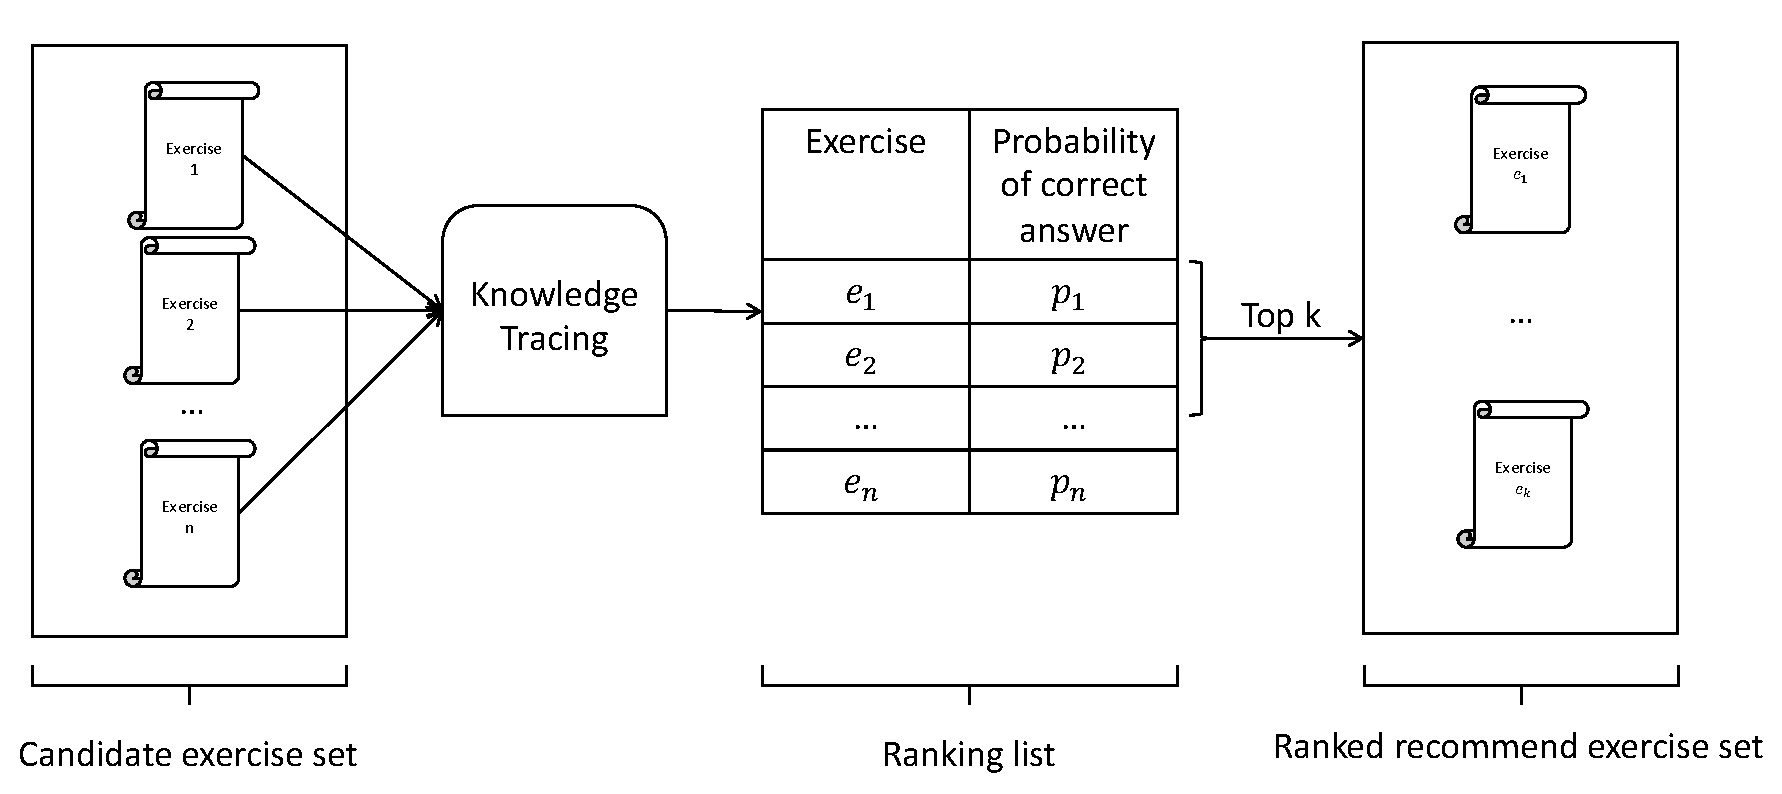
\includegraphics[width=0.9\textwidth]{ch4-model-ranking.pdf}
  \caption{The ranking method}\label{fig:ch4-model-ranking}
\end{figure}

%将候选集习题分别输入知识追踪模型得到预测值,即答对习题的概率,按照从小到大的顺序进行排序,筛选出前\(K_{Rank}\)项作为推荐习题列表。\(K_{Rank}\)为一个可调的超参数,它对于推荐结果影响较大,决定一道习题是否出现于最终的推荐列表中。当\(K_{Rank}\)较大时,推荐的准确率会更高,但是推荐效率会降低。在实际应用中,应当综合考虑学生的知识掌握水平与实际应用场景,设定合理的\(K_{Rank}\)值。

The last step of the model is to input the candidate's exercises into the knowledge tracing model to get the predicted value, that is, the probability of answering the exercises correctly. Sort them in ascending order, and filter out the top \(K_{Rank}\) items as a list of recommended exercises. \(K_{Rank}\) is an adjustable hyperparameter, which has a more significant impact on the recommendation result and determines whether an exercise will appear in the final recommendation list. When \(K_{Rank}\) is larger, the recommended accuracy rate will be higher, but the recommendation efficiency will be reduced. In practical applications, students' knowledge mastery level and practical application scenarios should be considered comprehensively, and a reasonable value of \(K_{Rank}\) should be set.

The general algorithm is as~\ref{alg:ch4-Rank}:
\begin{algorithm}[htbp!]
  \caption{Recommendation ranking algorithm}\label{alg:ch4-Rank}
  \begin{algorithmic}
    \REQUIRE~~\\
    The candidate exercises set \(\mathbf{E}^{(Candidate)}=\{E_1,E_2,\ldots,E_N\} \); \\
    \ENSURE~~\\ %算法的输出:Output
    The ranked recommendation exercise list \(\mathbf{E}^{(RANK)} \)
    \STATE~Input each exercises \(e_i \in \mathbf{E}^{(RANK)} \) to recommendation ranking model, i.e., knowledge tracing model, output the correct answering rate \(p_i\)
    \STATE~sort \(e_i \in \mathbf{E}^{(RANK)} \) by \(p_i\), output a ranked exercise list\(L\).
    \RETURN~~\(L[1..K_{RANK}]\) as \(\mathbf{E}^{(UCF)} \); %算法的返回值
  \end{algorithmic}
\end{algorithm}

\section{Experiments}
%本模型的核心思想是为学生查漏补缺,因此,在学生的知识状态一定的情况下,尽量给学生推荐对其知识掌握情况带来正向收益最大的习题。在实验阶段,一个基于公开知识追踪数据集的推荐数据集被生成出来,用来进行性能指标评估。

This model's core idea is to enhance students' proficiency in the parts with weak knowledge mastery. The model should recommend to students the exercises that bring the greatest positive benefits to their knowledge mastery. A recommended dataset based on the public knowledge tracing dataset is generated for performance evaluation in the experimental phase.
\subsection{Dataset}
%考虑到本推荐系统需要立足于学生的知识状态针对习题进行推荐,而目前市面上并没有专用的基于知识掌握度的数学习题推荐数据集,因此我们基于知识追踪数据集进行推荐数据集生成。本实验用了知识追踪领域的专用数据集ASSISTment 2009,它是一个用于预测学生考试表现的数据集,它由一系列包含若干知识点标签的问题以及一些学生的答题记录组成。它在2009-2010年于线上教育平台上采集而成。经过数据过滤获得包含4400个学生,110个知识点标签和约328291次交互次数的数据集。

Considering that this recommendation system needs to recommend exercises based on students' knowledge status, there is currently no dedicated dataset for mathematics exercise recommendations based on knowledge mastery proficiency. This model generates recommendation data sets based on the knowledge tracing dataset. This experiment uses the unique dataset ASSISTment2009 in the field of knowledge tracing. It is a dataset used to predict student test performance. It consists of a series of questions containing several knowledge point labels and some students' answer records. It was collected on the online education platform in 2009-2010. After data filtering, a dataset containing 4400 students, 110 knowledge point labels, and about 328,291 interaction times was obtained.

\subsection{Experiment Setting}
%原始数据集为一个固定的答题序列,为了衡量推荐效果,可以将当前时间戳\(t\)的回答习题\(q_t\)作为标定项,检查该习题是否存在于最终推荐结果中。由上一节的排序模型得出的最终推荐的输出为一个容量为\(K\)的列表,可以通过判定预测用户会答错的习题是否在该列表中的方法来判定模型的推荐效果。

The original data set is a fixed sequence of question-answering interaction. To measure the recommendation performance, the exercise \(q_t\) answered in timestamp \(t\) can act as the calibration item to check whether it is in the final recommendation result under the simultaneous state. The final recommendation output obtained by the ranking model in the previous section is a list with a capacity of \(K\), and the recommendation effect of the model can be determined by determining whether the exercises that predict the user will answer wrongly are in the list.

%本文的运行在环境如下表所示。在本实验的配置中,选择75\%的交互记录作为训练集,另外25\%作为测试数据。测试运行5次取平均值。实验取了三种不同的\(\tau \)作为习题正确率判断阈值。在推荐模型的召回阶段和排序阶段选取的超参数如表所示。

The running environment of this article is shown in Table~\ref{table:ch4-exp-env}. In this experiment's configuration, 75\% of the interaction records are selected as the training set and the remaining 25\% as the test dataset. Run the model 5 times and take the average. The hyperparameter settings of the recommendation model are shown in Table~\ref{table:ch4-hpsetting}. In the ranking stage, parameter \(N\) represents the number of Transformer stacking blocks in the knowledge tracing model, and \(d\) represents the sub-layer output's dimension.

\begin{table}[htbp!]
  \caption{Experiment running environment}\label{table:ch4-exp-env}
  \centering
  \begin{tabular}{l c}
    \toprule
    Software/Hardware & Configuration   \\
    \midrule
    CPU               & i7 9700K        \\

    GPU               & Tesla V100      \\

    Operating System  & Ubuntu 20.04    \\

    Python            & 3.8.6           \\

    PyTorch           & 1.6.0           \\

    GPU Driver        & Cuda10.1/cudnn7 \\
    \bottomrule
  \end{tabular}
\end{table}

\begin{table}[htbp!]
  \caption{Hyperparameter settings of recommendation model}\label{table:ch4-hpsetting}
  \centering
  \begin{tabular}{l c c}
    \toprule
    Parameter Belonging       & Hyperparameter     & Value \\
    \midrule
    \multirow{2}{*}{Collaborative filtering matching strategy}
                              & \(\tau^{simuser}\) & 0.9   \\
                              & \(K^{(UCF)}\)      & 10    \\
    \midrule
    \multirow{4}{*}{Popularity based matching strategy}
                              & \(w^{(SA)}\)       & 0.5   \\
                              & \(w^{(SF)}\)       & 0.1   \\
                              & \(w^{(SW)}\)       & 0.3   \\
                              & \(w^{(EX)}\)       & 0.1   \\
                              & \(K^{PMS}\)        & 10    \\
    \midrule
    \multirow{3}{*}{User preference based matching strategy}
                              & \(w^{(UW)}\)       & 0.9   \\
                              & \(w^{(UF)}\)       & 0.1   \\
                              & \(K^{UPM}\)        & 10    \\
    \midrule
    \multirow{4}{*}{Multiplex Merging}
                              & \(w^{(UCF)}\)      & 0.9   \\
                              & \(w^{(PMS)}\)      & 0.05  \\
                              & \(w^{(UPM)}\)      & 0.05  \\
                              & \(K^{(MERGE)}\)    & 10    \\
    \midrule
    \multirow{3}{*}{Ranking}  & \(K^{(RANK)}\)     & 10    \\
                              & \(N\)              & 3     \\
                              & \(d\)              & 256   \\
    \midrule
    \multirow{4}{*}{Training} & batch size         & 128   \\
                              & epochs             & 50    \\
                              & dropout rate       & 0.05  \\
                              & window size        & 100   \\
    \bottomrule
  \end{tabular}
\end{table}


\subsubsection{Baseline}
%作为对比,将目前较为热门的协同过滤推荐算法与随机推荐算法作为Baseline模型,协同过滤算法省略了matching阶段,直接寻找相似用户的习题作为推荐集合。而随机推荐算法则直接在习题库中随机选择习题进行推荐。

As a comparison, the more popular Collaborative Filtering (CF) recommendation algorithm and the random recommendation algorithm are used as Baseline models.
\begin{itemize}
  \item Collaborative Filtering: The collaborative filtering algorithm omits the matching stage and directly finds similar users' exercises as the recommendation set.
  \item Random: In each interaction, randomly determine whether the exercise will be recommended
\end{itemize}


\subsection{Metrics}
%本节提出的推荐模型的目标是向用户提出最符合当前知识状态的习题,因此推荐的精准度是一个关键的指标。为了更直观地显示推荐算法对于用户的知识提升作用,本实验将基于两个方面来进行模型性能判定。
%1. 推荐精准度判定:将知识追踪数据集的交互序列作为知识追踪模型的输入来训练模型。此时,运行推荐模型来生成一个习题推荐集合。记录学生\(s_i\)将序列中的时间\(t\)的习题\(e_{i,t}\)的推荐结果。如果知识追踪模型的对于习题\(e_{i,t}\)的预测概率低于一个判定阈值\(\tau\)时,表示该习题\(e_{i,t}\)对于学生\(s_i\)容易出错,因此应该被推荐。其混淆矩阵如下表


%排名低于\(K^{(RANK)}\),或者该习题在matching阶段即被淘汰,则不推荐该习题。
The goal of the recommendation model proposed in this section is to present the user with exercises that best match the current state of knowledge, so the accuracy of the recommendation is a key metric. In order to show more intuitively the knowledge enhancement effect of the recommendation algorithm on users, this experiment will be based on two aspects for model performance determination. Train the model by using the interaction sequence of the knowledge tracing dataset as the input of the knowledge tracing model. Simultaneously, the recommendation model is launched to generate a collection of exercise recommendations. Record the recommended results of the exercise \(e_{i,t}\) for which the student \(s_i\) will be in the sequence of time \(t\). If the prediction probability \(p_{i,t}\) of the knowledge-tracking model for the exercise \(e_{i,t}\) is lower than a given judgment threshold \(\tau \), it means that the exercise \(e_{i,t}\) is error-prone for the student \(s_i\) and thus should be recommended. The confusion matrix is:
\begin{itemize}
  \item True Positive(TP): exercise \(e_{i,t}\) is in output recommendation exercise set and \(p_{i,t}<\tau \)
  \item True Positive(FP): exercise \(e_{i,t}\) is in output recommendation exercise set and \(p_{i,t}\geq \tau \)
  \item True Positive(FN): exercise \(e_{i,t}\) is not in output recommendation exercise set and \(p_{i,t}<\tau \)
  \item True Positive(TN): exercise \(e_{i,t}\) is not in output recommendation exercise set and \(p_{i,t}\geq \tau \)
\end{itemize}
Where \(\tau \) is an adjustable hyperparameter, this is a classification problem, so the Receiver Operator Characteristic Curve (ROC) curve can be used to determine the performance of the recommendation system. Then, (Area Under Curve) AUC and Accuracy (ACC) metrics can be used to determine the performance of the model.

\subsection{Result and Analysis}
Five different \(\tau \) (0.45, 0.5, 0.55) are applied as the threshold for judging the predicting correctness of the exercises. The result is shown in \tblname{\ref{table:ch4-exp-result}}. %~\ref{table:ch4-exp-result}.
\begin{table}[htbp!]
  \caption{Recommendation experiment result}\label{table:ch4-exp-result}
  \centering
  \begin{tabular}{c c c}
    \toprule
    Model                    & ACC    & AUC    \\
    \midrule
    CF                       & 0.5375 & 0.5239 \\
    Random                   & 0.5073 & 0.5012 \\
    \midrule
    Proposed \((\tau=0.45)\) & 0.6542 & 0.6878 \\
    Proposed \((\tau=0.50)\) & 0.6839 & 0.7375 \\
    Proposed \((\tau=0.55)\) & 0.6657 & 0.7039 \\
    \bottomrule
  \end{tabular}
\end{table}
%经过对比,我们发现,基于知识追踪模型进行的习题推荐,在ACC和AUC指标上都大幅超越Baseline算法,这说明了提出的模型可以有效筛选出对于学生知识状态增益较大的习题集合,从而实现基于学生的学习状态进行自适应习题推荐。
After comparison, it can be concluded that the knowledge tracing model-based exercise recommendation significantly outperforms the Baseline algorithm in both ACC and AUC metrics, which indicates that the proposed model can effectively filter out the set of exercises with greater gain for students' knowledge state, thus realizing adaptive exercise recommendation based on students' learning state.

\section{Summary}
%本章提出一个基于Matching-Ranking双阶段的数学习题推荐模型。其中第一阶段的Matching模型为一个多路习题推荐项匹配模型,该模型采用了基于协同过滤、热门度、用户偏好等多个子召回策略用于分别生成习题推荐候选集合,然后在融合阶段将这些候选集合进行加权融合,形成一个最终的融合习题推荐候选集合。在排序阶段,将Matching阶段获取的习题候选集合中的每个习题输入到知识追踪习题进行正确率预测,将最容易出错的习题的作为优先级最高的推荐项,按照此策略生成推荐习题集。
%本章的主要贡献有两点:
%1.将多路召回策略应用于习题的Matching阶段,从而可以利用相对小的计算负载来快速筛选出候选习题集,所有的习题在不同的策略中有不同的推荐分,按照推荐分从高到低的顺序,取前若干个习题作为候选集合。对于不同的策略,可以动态调节它们的权重,来实现对于推荐侧重点的人工控制。
%2.将习题输出前一章提出的知识追踪模型,将模型输出的习题正确率作为习题的推荐分依据。这种机制将学生最可能答错的习题推荐给学生,从而加强学生对于知识掌握水平较低的知识点的理解。

In this chapter, a two-stage Matching-Ranking based mathematical exercise recommendation model is proposed. The Matching model in the first stage is a multiplexed exercise recommendation item matching model, which employs multiple sub-matching strategies based on collaborative filtering, popularity, user preferences for generating exercise recommendation candidate sets separately, and then these candidate sets are weighted and fused in the fusion stage to form a final fused exercise recommendation candidate set. In the ranking phase, each exercise in the set of exercise candidates obtained in the Matching phase is input to the knowledge tracing exercise for correctness prediction, and the most error-prone exercises are used as the recommendation item with the highest priority, and the recommended set of exercises is generated according to this strategy.
The main contribution of this chapter is:
\begin{enumerate}
  \item The multiple matching strategies are applied to the Matching stage of the exercises so that the candidate set of exercises can be filtered quickly with a relatively small computational load and all the exercises have different recommendation scores in different strategies. For different strategies, their weights can be dynamically adjusted to achieve manual control over the recommendation focus.
  \item The knowledge tracing model proposed in the previous chapter is outputted for the exercises, and the correctness of the model output is used as the basis for the recommended score for the exercises. This mechanism recommends the exercises that students are most likely to answer incorrectly, thus enhancing students' understanding of the knowledge points with lower levels of knowledge mastery proficiency.
\end{enumerate}